\section{Results}
\label{sec:results}

\paragraph{Family-conditional hardness (completed bench).}
On the fitted DenoiseOpt $100{,}000$-cycle bench, denoise score $D$ is lowest for \texttt{nonlinear} ($D\approx 0.39$) and \texttt{combo} ($D\approx 0.40$), then \texttt{triple\_mix} / \texttt{extreme\_overlay} ($D\approx 0.51$--$0.52$), while \texttt{harmonic\_fft} and \texttt{am\_fm} sit near $D\approx 0.69$--$0.70$.
Lit-combo champion family stress (prolonged residual) similarly ranks \texttt{open\_wrap\_bias} ($R\approx 0.83$) and \texttt{extreme\_overlay} / \texttt{combo} ($R\approx 0.88$--$0.89$) below \texttt{harmonic\_fft} ($R\approx 0.95$).
Hard sounds recur.

\paragraph{Overnight hybrid ($5$k-gate freeze).}
At $\ge 5{,}000$ clean iterations the champion residual is $R\approx 0.99093$ with DualCosine $\approx 0.81658$ on the overnight runner ($\Delta R\approx{+}0.174$).
Monitoring plots below are regenerated from that freeze.
Declared larger budgets continue. This paper reports the gate freeze only.

\paragraph{Inference time at matched score.}
Across diverse high-$R$ fitted cells ($R\ge 0.98$), we timed CUDA forward passes (batch 64, prolonged residual).
Within a tight band of the best residual ($R \ge R_{\max}-5\cdot10^{-4}$), the \textbf{favorite} is the lowest-latency model:
\texttt{champion\_iter\_000235} with $R\approx 0.9910$, $\approx 3.15$\,ms/batch, $\approx 37$k parameters
(versus a higher-capacity max-$R$ cell at $R\approx 0.9914$ but $\approx 7.18$\,ms/batch / $\approx 104$k params).
Selection rule: maximize $R$, then minimize latency inside the band.

\subsection{Top-5 architectures}
\label{sec:top5-arch}
Table~\ref{tab:top5} ranks five distinct fitted bake graphs from the CUDA inference bench
(\texttt{inference\_bench.json}, batch 64), preferring residual $R$ first and latency on ties,
and skipping near-duplicate copies of the same topology signature.

\begin{table}[t]
  \centering
  \caption{Top-5 distinct fitted architectures on the CUDA inference bench (batch 64, prolonged $R$, seed geometry matching overnight). Favorite is latency-best inside the near-max-$R$ band ($R\ge R_{\max}-5\cdot10^{-4}$).}
  \label{tab:top5}
  \setlength{\tabcolsep}{3pt}
  \begin{tabular}{@{}lrrrr@{}}
    \toprule
    Tag & $R_{\mathrm{saved}}$ & $R_{\mathrm{live}}$ & ms/batch & params \\
    \midrule
    \texttt{iter\_000157} & 0.9914 & 0.9913 & 7.18 & 104\,484 \\
    \texttt{iter\_000205} & 0.9911 & 0.9907 & 7.29 & 70\,562 \\
    \texttt{iter\_000235}* & 0.9910 & 0.9915 & 3.15 & 37\,489 \\
    \texttt{iter\_000397} & 0.9910 & 0.9907 & 6.80 & 97\,262 \\
    \texttt{iter\_000229} & 0.9909 & 0.9902 & 6.67 & 100\,500 \\
    \bottomrule
  \end{tabular}\\[0.4em]
  {\footnotesize *Favorite (fastest in $R\ge R_{\max}-5\cdot10^{-4}$ band).}
\end{table}

\paragraph{Classical vs favorite (canonical holdout).}
Table~\ref{tab:canonical-methods} scores the classical bake set plus DualCosine and the neural favorite on the frozen corpus of Section~\ref{sec:dataset} (CUDA, batch 64, seed $20{,}260{,}719$).
DualCosine reaches $R\approx 0.825$ ($\approx 1.35$\,ms/batch), near the overnight monitor DualCosine $\approx 0.817$ on live draws from the same generator.
The best \emph{active} classical method is seam-local 3-tap FIR (\texttt{seam\_fir3}) at $R\approx 0.961$ / $\approx 0.67$\,ms/batch ($0.962\pm0.002$ over five seeds).
Identity (no-op) scores $R\approx 0.972$ and is a ceiling only.
The neural favorite reaches $R\approx 0.991$ ($0.991\pm0.0002$ over five seeds) at $\approx 2.56$\,ms/batch ($\approx 37$k params): $\Delta R \approx {+}0.030$ vs \texttt{seam\_fir3} and $\Delta R \approx {+}0.166$ vs DualCosine.

\begin{table}[t]
  \centering
  \caption{Method scores on the canonical sine{+}cliff holdout (batch 64, seed $20{,}260{,}719$, $L{=}256$, $N{=}16$). Mean$\pm$std over five consecutive seeds. Identity is a no-op ceiling. Primary metric is prolonged $R$ (1~=~best).}
  \label{tab:canonical-methods}
  \setlength{\tabcolsep}{3pt}
  \begin{tabular}{@{}lrrr@{}}
    \toprule
    Method & $R$ & $R$ (5-seed) & ms/batch \\
    \midrule
    neural favorite & 0.9911 & $0.9912\pm0.0002$ & 2.56 \\
    identity (no-op) & 0.9718 & $0.9726\pm0.0021$ & 0.31 \\
    \texttt{seam\_fir3} & 0.9610 & $0.9616\pm0.0019$ & 0.67 \\
    classic quadratic & 0.8449 & $0.8453\pm0.0117$ & 1.59 \\
    DualCosine & 0.8249 & $0.8258\pm0.0137$ & 1.35 \\
    cosine fade & 0.8249 & $0.8258\pm0.0137$ & 1.59 \\
    crossfade & 0.8116 & $0.8130\pm0.0145$ & 1.50 \\
    hann blend & 0.8048 & $0.8060\pm0.0156$ & 0.54 \\
    soft wide fade & 0.7432 & $0.7378\pm0.0171$ & 2.64 \\
    detrend & 0.4079 & $0.4091\pm0.0386$ & 0.36 \\
    ensemble detrend{+}DC{+}FIR & 0.4024 & $0.4027\pm0.0387$ & 1.56 \\
    \bottomrule
  \end{tabular}
\end{table}

\subsection{SOTA matrix skeleton (frozen holdout)}
\label{sec:sota-skeleton}

Table~\ref{tab:sota-main} is the Phase~4 skeleton built from existing \texttt{method\_scores.json}.
Columns for SNR, SDR, and wrap-jump await Phase~3a metric plumbing on the same tensors.
PESQ/STOI are intentionally omitted (non-speech cycles).

\begin{table}[t]
  \centering
  \caption{SOTA comparison skeleton on the frozen sine{+}cliff holdout (seed $20{,}260{,}719$, batch 64). $R$ and latency from \texttt{method\_scores.json}. $\Delta R$ is vs DualCosine on the same freeze. SNR/SDR/wrap-jump columns deferred to Phase~3a.}
  \label{tab:sota-main}
  \setlength{\tabcolsep}{2.5pt}
  \begin{tabular}{@{}lrrrr@{}}
    \toprule
    Method & $R$ & $\Delta R$ vs DC & ms/batch & params \\
    \midrule
    neural favorite & 0.9911 & ${+}0.1662$ & 2.56 & 37\,489 \\
    identity & 0.9718 & ${+}0.1469$ & 0.31 & 0 \\
    \texttt{seam\_fir3} & 0.9610 & ${+}0.1361$ & 0.67 & 0 \\
    classic quadratic & 0.8449 & ${+}0.0200$ & 1.59 & 0 \\
    DualCosine & 0.8249 & $0$ & 1.35 & 0 \\
    cosine fade & 0.8249 & $0$ & 1.59 & 0 \\
    crossfade & 0.8116 & ${-}0.0133$ & 1.50 & 0 \\
    hann blend & 0.8048 & ${-}0.0201$ & 0.54 & 0 \\
    soft wide fade & 0.7432 & ${-}0.0817$ & 2.64 & 0 \\
    detrend & 0.4079 & ${-}0.4170$ & 0.36 & 0 \\
    ensemble DC+FIR & 0.4024 & ${-}0.4225$ & 1.56 & 0 \\
    \bottomrule
  \end{tabular}
\end{table}

\begin{figure}[t]
  \centering
  
\includegraphics[width=\columnwidth]{figures/fig_inference_vs_residual.png}
  \caption{High-$R$ fitted cells on CUDA (batch 64): prolonged residual $R$ versus forward latency (ms/batch). Star marks the favorite (fastest inside the near-max-$R$ band).}
  \label{fig:inference-pareto}
\end{figure}

\begin{figure}[t]
  \centering
  
\includegraphics[width=\columnwidth]{figures/fig_inference_latency_bars.png}
  \caption{Inference latency (ms/batch, CUDA, batch 64) for diverse high-$R$ fitted models from the inference bench.}
  \label{fig:inference-bars}
\end{figure}

\begin{figure}[t]
  \centering
  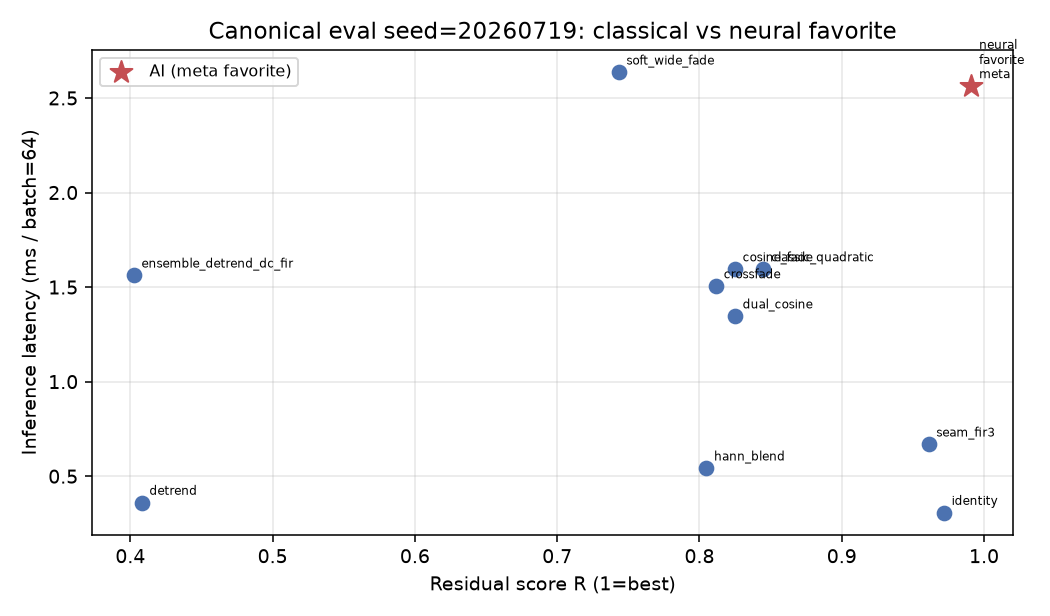
\includegraphics[width=\columnwidth]{figures/fig_classical_vs_ai_scatter.png}
  \caption{Canonical holdout (seed $20{,}260{,}719$, batch 64): classical bake methods and neural favorite in the $R$ vs CUDA ms/batch plane. Star: favorite.}
  \label{fig:classical-vs-ai-scatter}
\end{figure}

\begin{figure}[t]
  \centering
  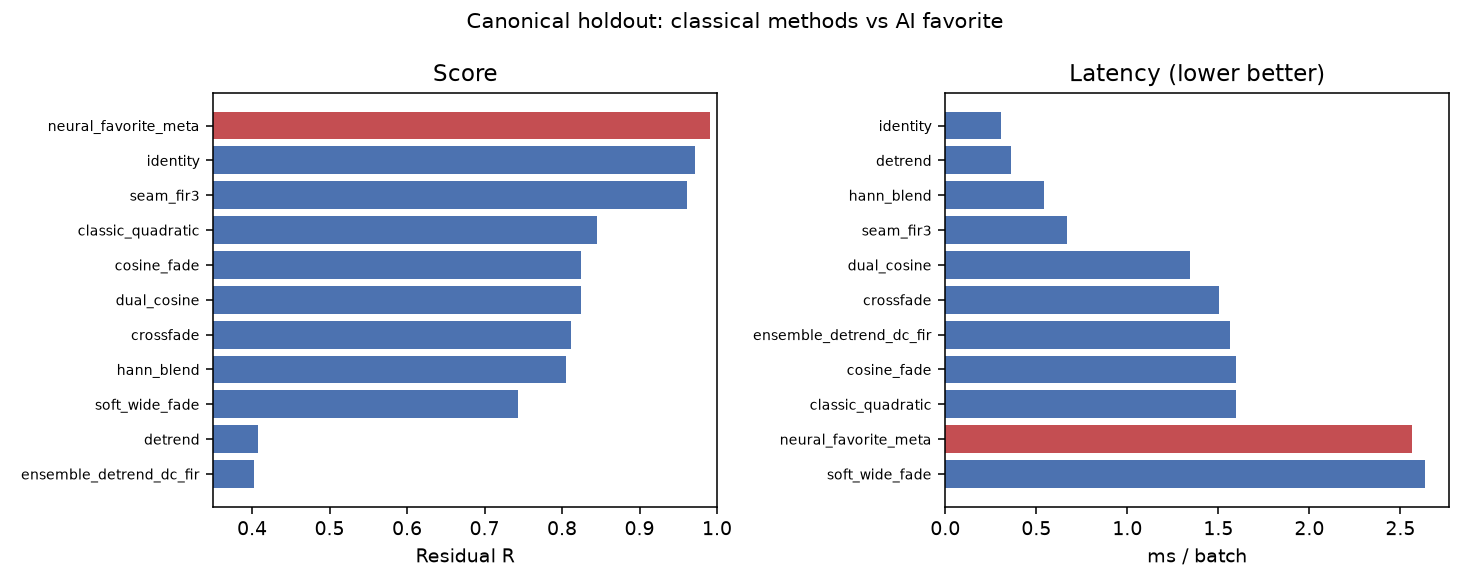
\includegraphics[width=\columnwidth]{figures/fig_classical_vs_ai_bars.png}
  \caption{Canonical holdout ranking on prolonged residual $R$ (left) and CUDA latency (right). DualCosine $R\approx 0.825$. Favorite highlighted.}
  \label{fig:classical-vs-ai-bars}
\end{figure}

\begin{figure}[t]
  \centering
  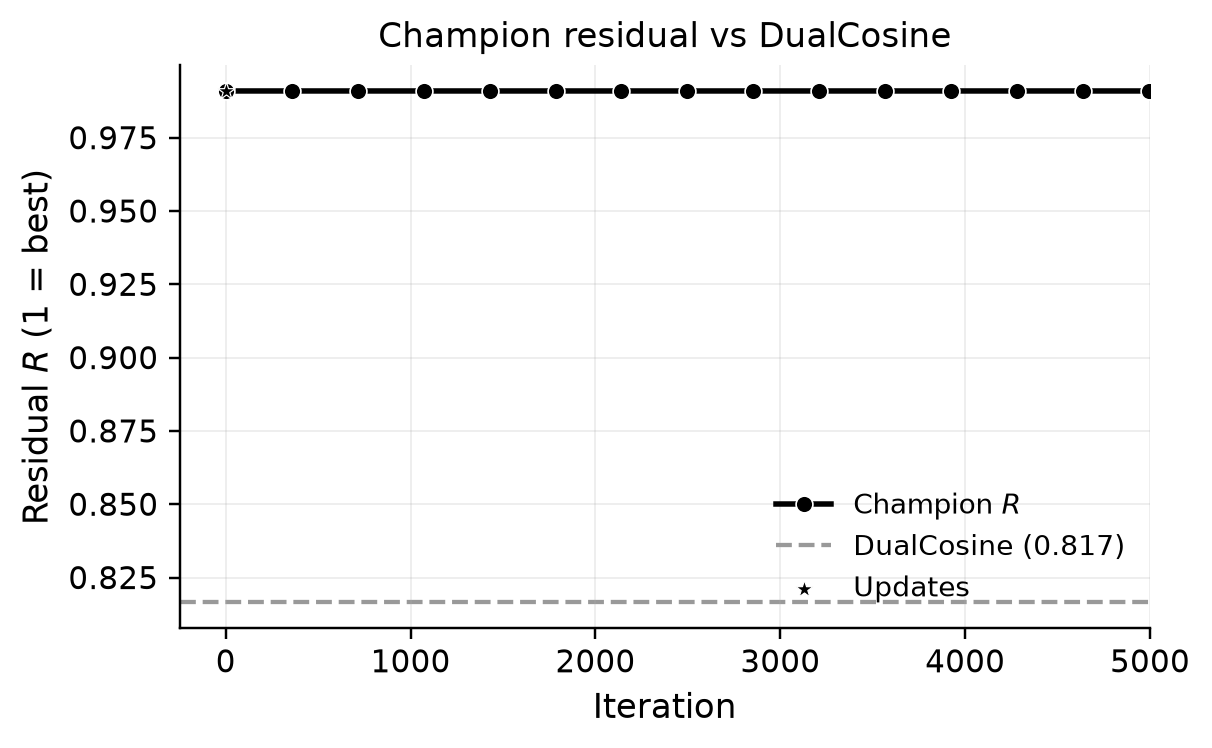
\includegraphics[width=\columnwidth]{figures/champ_residual_vs_iter.png}
  \caption{Overnight $5$k-gate freeze: champion residual $R$ versus clean search iteration, with DualCosine baseline on the runner geometry (RTX~3090).}
  \label{fig:champ-residual}
\end{figure}

\begin{figure}[t]
  \centering
  
\includegraphics[width=\columnwidth]{figures/branch_bests_vs_iter.png}
  \caption{Overnight $5$k-gate freeze: per-branch best residual trajectories (PPO/RL, GA, PBT, NAS, combo) versus iteration.}
  \label{fig:branch-bests}
\end{figure}

\begin{figure*}[t]
  \centering
  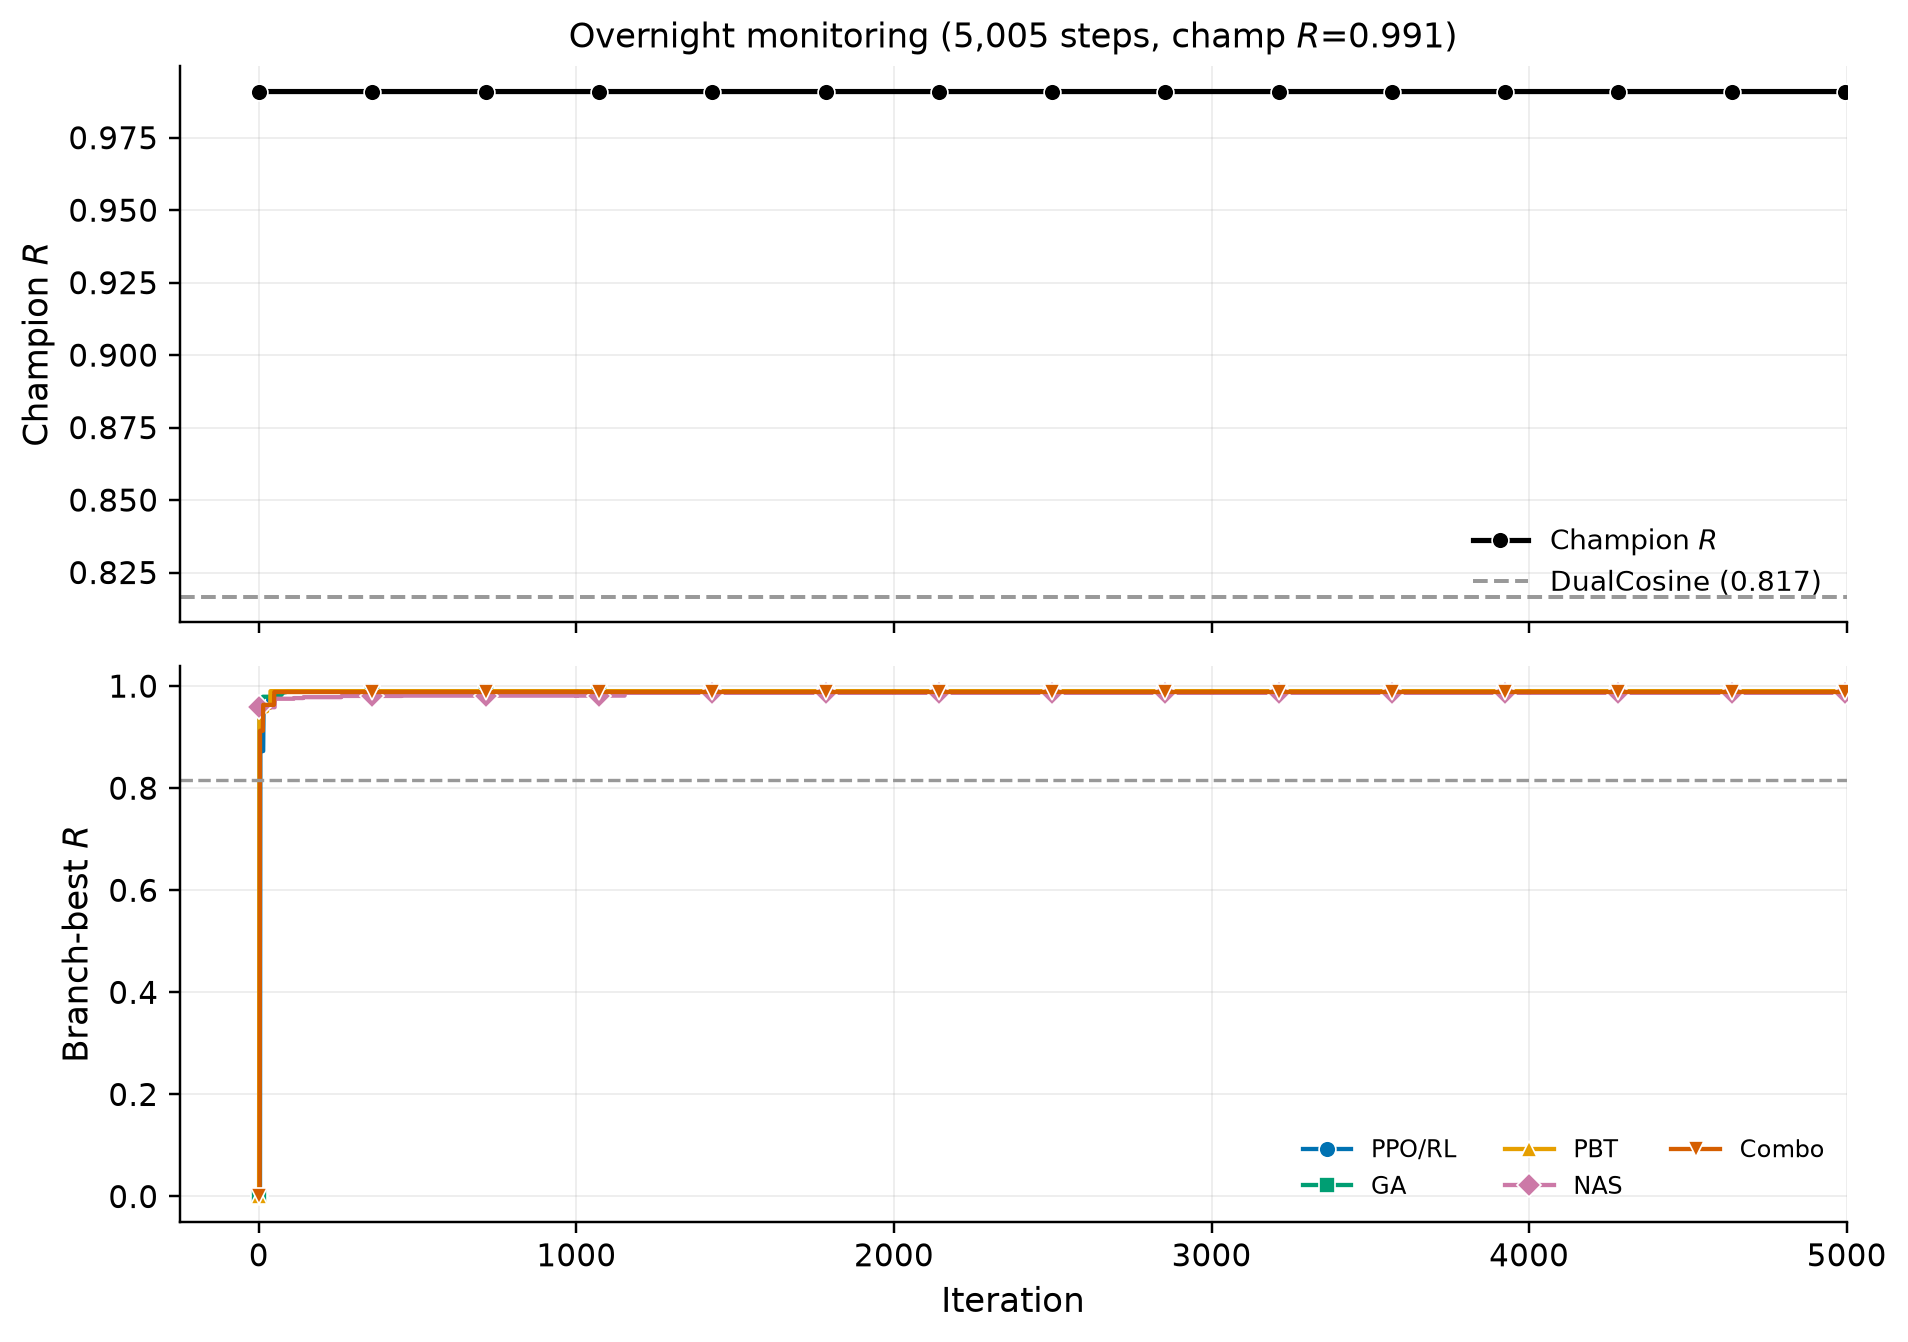
\includegraphics[width=\textwidth]{figures/overnight_panel.png}
  \caption{Full-width overnight monitoring panel at the $5$k-gate freeze: champion $R$ (top) and branch-best trajectories (bottom). Source: \texttt{history.jsonl} regenerated figures.}
  \label{fig:overnight-panel}
\end{figure*}

\begin{figure}[t]
  \centering
  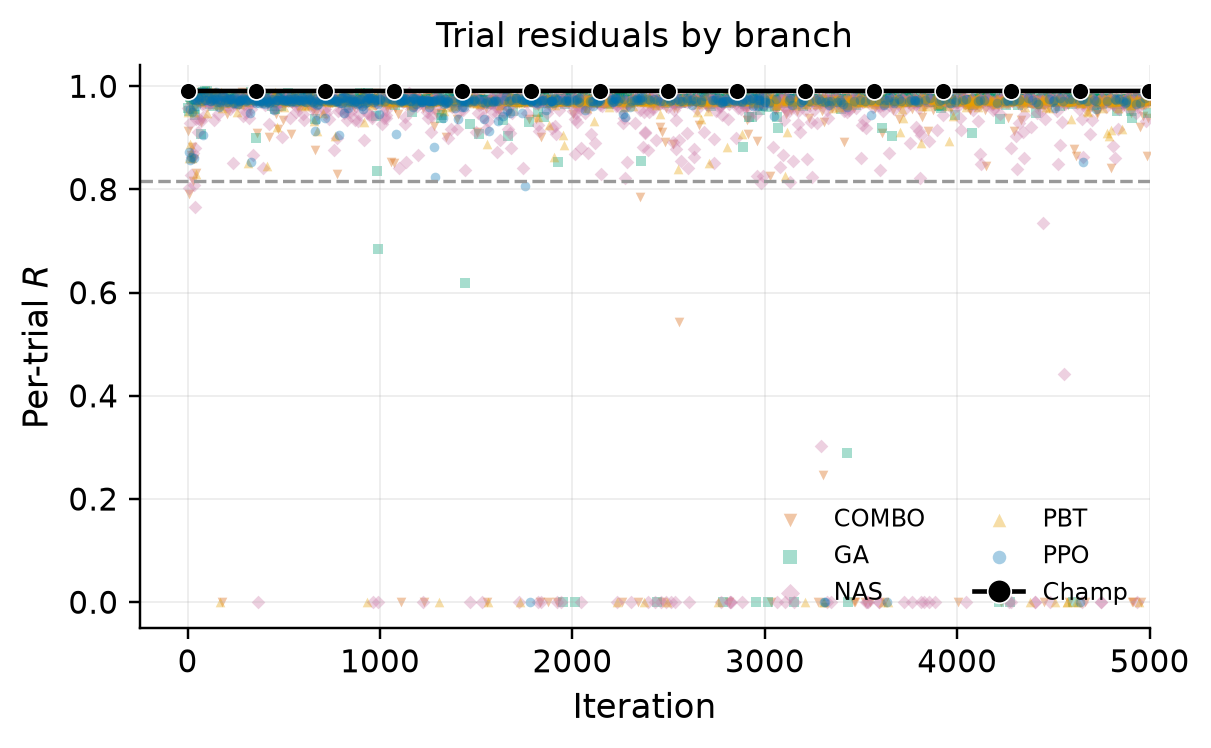
\includegraphics[width=\columnwidth]{figures/residual_by_branch.png}
  \caption{Per-trial residual scatter by search branch at the $5$k-gate freeze, with champion overlay.}
  \label{fig:residual-branch}
\end{figure}

\begin{figure}[t]
  \centering
  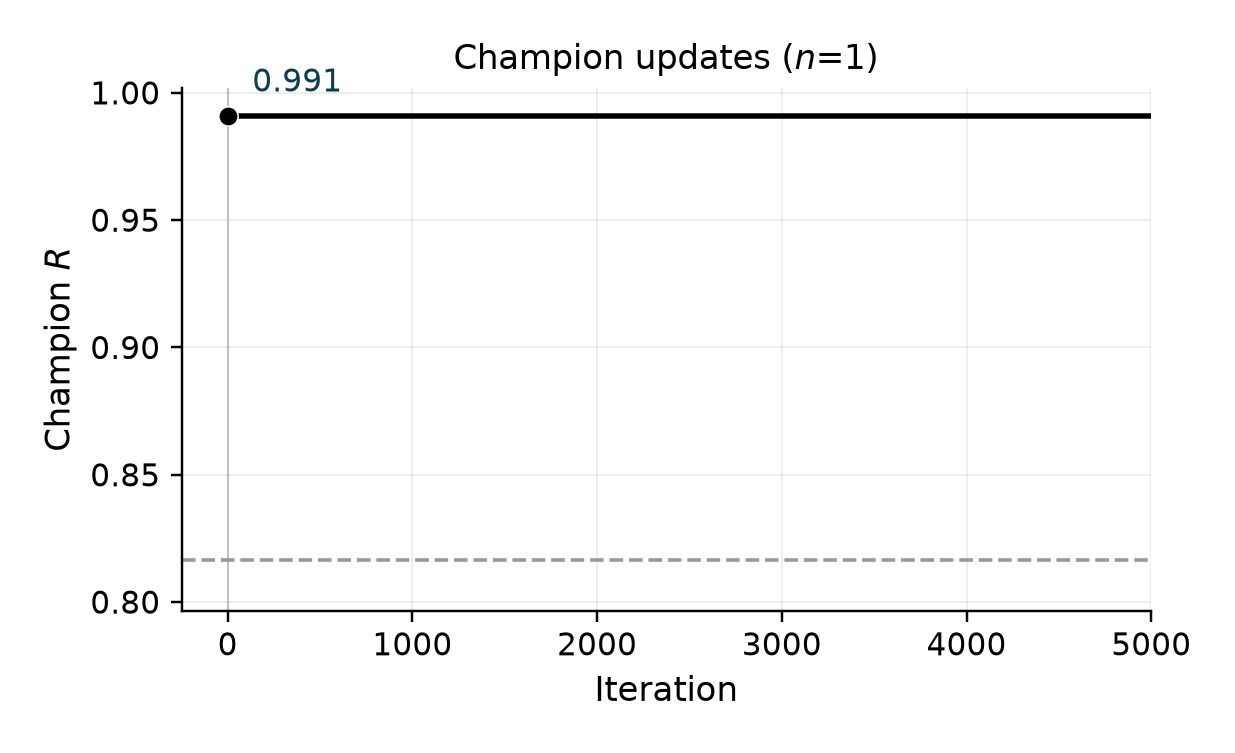
\includegraphics[width=\columnwidth]{figures/champion_timeline.png}
  \caption{Champion update timeline at the $5$k-gate freeze. Sparse $R$ labels mark first, mid-peak, and latest improvements for twocolumn legibility.}
  \label{fig:champ-timeline}
\end{figure}
